\documentclass[12 pt,a4paper]{report}
\setlength{\topmargin}{-2cm}
\setlength{\oddsidemargin}{0cm}
\setlength{\textheight}{24cm}
\setlength{\textwidth}{16cm}

\usepackage{graphicx}



%Use sffamily for all titles


\begin{document}

\title{\sffamily\huge\textbf{Report on Sorting Algorithms}}
\author{Kavi Zahan Sultana}
\date{01/12/2014}
\maketitle


\newpage

\tableofcontents

\newpage

\section{Introduction}

This report provides the introduction, algorithm,running time and graphs of sorting algorithms.

\section{Insertion Sort}

Insertion sort is an efficient algorithm for sorting a small number of elements. We present the pseudocode called INSERTION-SORT.
It takes as a parameter an array /textit{A[1..n]}  containing a sequence of length \textit{n} that is to be sorted.

\subsection{Algorithm}

$INSERTION-SORT(A)$

1   \textbf{for}  $j=2   \textbf{   to  }   A.length$

2    \hspace{1cm}$ key=A[j] $

3     \hspace{1cm}$i=j-1$

4     \hspace{1cm}$\textbf{while  }i>0\hspace{0.3cm}and \hspace{0.3cm} A[i]>key$

5     \hspace{1.5cm}$A[i+1]=A[i]$

6     \hspace{1.5cm}$i=i-1$

7     \hspace{1cm}$A[i+1]=key$


\subsection{ Time Complexity  of  Insertion  Sort}

$INSERTION-SORT(A)  \hspace{3cm}cost \hspace{1cm}times$
\vspace{0.4cm}

1\hspace{0.75cm}$\textbf{for}\hspace{0.3cm}j=2 \textbf{ to } A.length\hspace{2.5cm}c_1\hspace{1cm} n  $

2\hspace{1.5cm}$key=A[j]\hspace{3.94cm}c_2\hspace{1cm}n-1$

3\hspace{1.5cm}$i=j-1\hspace{4.2cm}c_3\hspace{1cm}n-1$

4\hspace{1.5cm}$\textbf{while }i>0 and A[i]>key\hspace{1.1cm}c_4\hspace{1cm}\sum_{j=2}^nt_j$

5\hspace{2cm}$A[i+1]=A[i]\hspace{2.7cm}c_5\hspace{1cm}\sum_{j=2}^n(t_j-1)$

6\hspace{2cm}$i=i-1\hspace{3.8cm}c_6\hspace{1cm}\sum_{j=2}^n(t_j-1)$

7\hspace{1.5cm}$A[i+1]=key\hspace{3.3cm}c_7\hspace{1cm}n-1$


\vspace{1.5cm}



The running time of the algorithm is the sum of running times for each statement executed.To compute $T(n)$, the  running time of $INSERTION-SORT$ on an input of \textit{n} values, we sum the products of the \textit{cost} and \textit{times} columns,obtaining\\

$T(n)=c_1n+c_2(n-1)+c_3(n-1)+c_4\sum_{j=2}^nt_j + c_5\sum_{j=2}^n(t_j-1)+ c_6\sum_{j=2}^n(t_j-1) + c_7(n-1)$\\

\textbf{1.Best case:}

In $INSERTION-SORT$, the best case occurs if the array is already sorted. For each$ j=2,3,...,n$, we then find that $A[i]<=key$ in line 5 when \textit{i} has its initial value of $j-1$. Thus $t_j=1$ for $ j=2,3,...,n$, and the best-case running time is\\

$T(n)=c_1n+c_2(n-1)+c_3(n-1)+c_4(n-1) + c_7(n-1)$\\

\hspace{1cm}$=(c_1+c_2+c_3+c_4+c_7)n-(c_2+c_3+c_4+c_7).$\\

\hspace{1cm}$=an+b$\\

where, $a=(c_1+c_2+c_3+c_4+c_7)$ and $b=-(c_2+c_3+c_4+c_7)$, which depend on the statement costs $c_i$; it is thus a \textbf{\textit{linear function}} of \textit{n}.\\

\newpage

\textbf{2.Worst case:}

If the array is in reverse sorted order-that is, in decreasing order- the worst case results.We must compare each element $A[j]$ with each element in the entire sorted subarray$A[1..j-1]$, and so $t_j=j$ for $j=2,3,...,n$. Noting that \\

$\sum_{j=2}^nj=n(n+1)/2-1$\\

and\\

$\sum_{j=2}^n(j-1)=n(n-1)/2$\\

Therefore, in worst case, the running time of $INSERTION-SORT$ is\\
$$\hspace{0.5cm}T(n)=c_1n+c_2(n-1)+c_3(n-1)+c_4(n(n+1)/2-1)+c_5(n(n-1)/2)+ c_6(n(n-1)/2)+c_7(n-1)$$
$$\hspace{1.5cm}=(c_4/2+c_5/2+c_6/2)n^2+(c_1+c_2+c_3+c_4/2-c_5/2-c_6/2+c_8)n-(c_2+c_3+c_4+c_7)$$
$\hspace{1.5cm}=an^2+bn+c$\\

which is a \textbf{\textit{ quadratic equation}}. Here,$an^2+bn+c$ for constants a,b and c that again depend on the statement costs $c_i$; it is thus a \textbf{\textit{quadratic function}} of \textit{n}.\\
\newpage


\textbf{3.Average  case:}\\

The \textbf{average case} is often roughly as bad as the worst case. On average half the elements in $A[1..j-1]$ are less than $A[j]$,and half the elements are greater. On average, therefore, we check half of the subarray $A[1..j-1]$, and so $t_j$ is about $j/2$. The resulting average case running time turns out to be a quadratic function of the input size, just like the worst-case running time.

Here is the chart of time complexity of insertion sort.

\vspace{1cm}

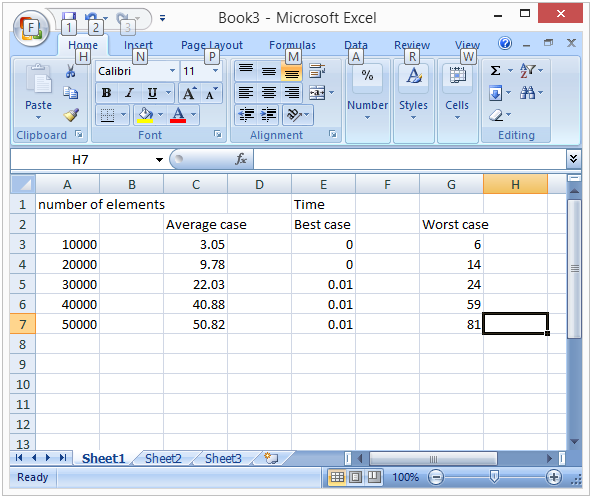
\includegraphics{insertdata.png}

\hspace{5cm}fig: Chart of Insertion Sort.

\subsection{Graph of Time Complexity of Insertion Sort}

Here is the graph of  comparison of running times of average case,best case and worst case.\\


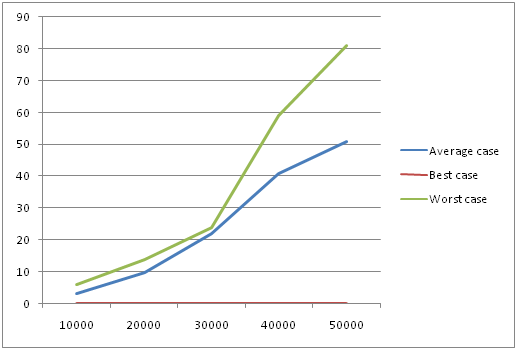
\includegraphics{img-1.png}

\hspace{4cm}fig: time vs n graph for insertion sort.

\newpage

\section{Merge Sort}

The \textbf{\textit{Merge Sort}} algorithm closely follows the divide and conquer paradigm. Intuitively, it operates as follows,
\vspace{0.5cm}

\textbf{Divide:}

Divide the \textit{n}- element sequence to be sorted into two subsequences of $n/2$ elements  each.
\vspace{0.5cm}

\textbf{Conquer:}

Sort the two subsequences recursively using merge sort.
\vspace{0.5cm}

\textbf{Combine:}

Merge the two sorted subsequences to produce the sorted answer.
\vspace{0.5cm}

The key operation of the merge sort algorithm is the merging of two sorted sequences in the \textbf{combine} step. We merge by calling an auxiliary procedure $MERGE(A,p,q,r)$, where \textit{A} is an array and \textit{p,q} and \textit{r} are indices into the array such that $p\leq q<r$. The procedure assumes that the subarray $A[p..q]$ and $A[q+1..r]$ are in sorted order. It \textbf{\textit{merges}} them to form a single sorted subarray that replaces the current subarray $A[p..r]$.
\vspace{0.5cm}

Our $MERGE$ procedure takes time $\Theta(n)$, where $n=r-p+1$ is the total number of elements being merged.

\newpage


\subsection{Algorithm}

The following pseudocode implements $MERGE(A,p,q,r)$ procedure, which merges the two subsequences. And another pseudocode $MERGE-SORT(A,p,r)$ sorts the elements in the subarray$A[p..r]$.
\vspace{1cm}

$MERGE(A,p,q,r)$


1\hspace{0.5cm} $n_1=q-p+1$


2\hspace{0.6cm}$n_2=r-q$


3\hspace{0.6cm}//create arrays $L[1...n_1+1]$ and $R[1...n_2+1]$.


4\hspace{0.6cm}$\textbf{for } i=1\hspace{0.2cm}to \hspace{0.2cm}n_1$


5\hspace{1cm}$do\hspace{0.2cm}L[i]=A[p+i-1]$

6\hspace{0.6cm}$\textbf{for}\hspace{0.2cm} j=1\hspace{0.2cm}to\hspace{0.2cm}n_2$

7\hspace{1cm}$do\hspace{0.2cm} R[j]=A[q+j]$

8\hspace{0.6cm}$L[n_1+1]=\infty$

9\hspace{0.6cm}$R[n_2+1]=\infty$

10\hspace{0.5cm}$i=1$

11\hspace{0.5cm}$j=1$

12\hspace{0.5cm}$\textbf{for}\hspace{0.2cm}k=p\hspace{0.2cm}to\hspace{0.2cm}r$

13\hspace{1cm}$do\hspace{0.2cm}if\hspace{0.2cm}L[i]\leq R[j]$

14\hspace{1.5cm}$then\hspace{0.2cm}A[k]=L[i]$

15\hspace{1.5cm}$i=i+1$

16\hspace{1cm}$else\hspace{0.3cm}A[k]=R[j]$

17\hspace{1.5cm}$j=j+1$

\vspace{1cm}

$MERGE-SORT(A,p,r)$

1\hspace{0.5cm}$\textbf{if}\hspace{0.2cm}p<r$

2\hspace{1cm}$q=\left [(p+r)/2\right]$

3\hspace{1cm}$MERGE-SORT(A,p,q)$

4\hspace{1cm}$MERGE-SORT(A,q+1,r)$

5\hspace{1cm}$MERGE(A,p,q,r)$

\subsection{Time Complexity of MERGE-SORT}

\vspace{1cm}

There are no such differences among the best,worst and average case of time complexity in merge sort.

\textbf{Best case:} In best case, the running time of merge sort is,$T(n)=O(nlog(n))$.
\vspace{0.5cm}

\textbf{Average case:} In average case, the running time of merge sort is, $T(n)=O(nlog(n))$.
\vspace{0.3cm}

\textbf{Worst case:} In worst case, the running time of worst case is, $T(n)=O(nlog(n))$.

Here, is the chart of time complexity in merge sort-

\vspace{1cm}

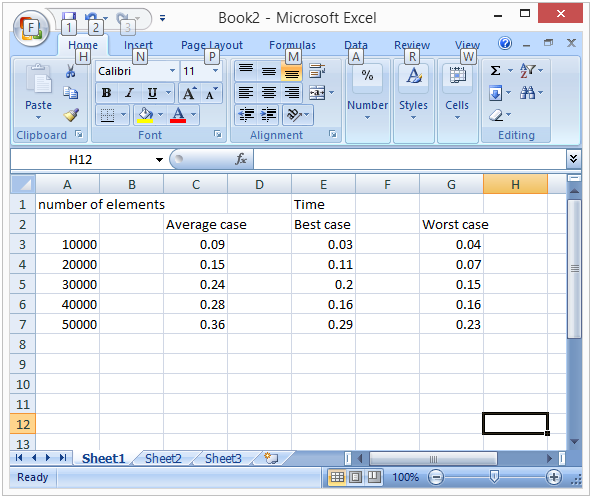
\includegraphics{mergedata.png}

\hspace{5cm}fig: Time Complexity chart.

\subsection{Graph of Time Complexity of MERGE-SORT}

We can represent time complexity of $MERGE-SORT$ by the following graph.


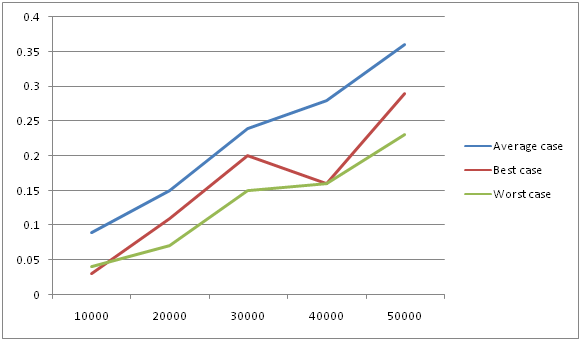
\includegraphics{mergesort.png}

\hspace{5cm}fig: Time complexity  graph  of merge sort.

\section{Bubble Sort}



\textbf{Bubble Sort} is a popular, but inefficient, sorting algorithm. It works by repeatedly swapping adjacent elements that are out of order.

\subsection{Algorithm of BUBBLE SORT}

\vspace{1cm}

$BUBBLE-SORT(A)$

1\hspace{0.5cm}$\textbf{for}\hspace{0.2cm}i=1\hspace{0.2cm}to\hspace{0.2cm}length[A]$

2\hspace{1cm}$do\hspace{0.2cm}\textbf{for}\hspace{0.2cm}j=length[A]\hspace{0.2cm}downto\hspace{0.2cm}i+1$

3\hspace{1.5cm}$do\hspace{0.2cm}\textbf{if}\hspace{0.2cm}A[j]<A[j-1]$

4\hspace{2cm}$then\hspace{0.2cm}exchange\hspace{0.2cm}A[j]<->A[j-1]$

\subsection{Time Complexity of BUBBLE SORT}

 In  average and worst case, the running time of BUBBLE-SORT are same, $T(n)=O(n^2)$. But in best case, the running time is $O(n)$.

\vspace{1cm}

Here is the table of time complexity-

\vspace{1cm}

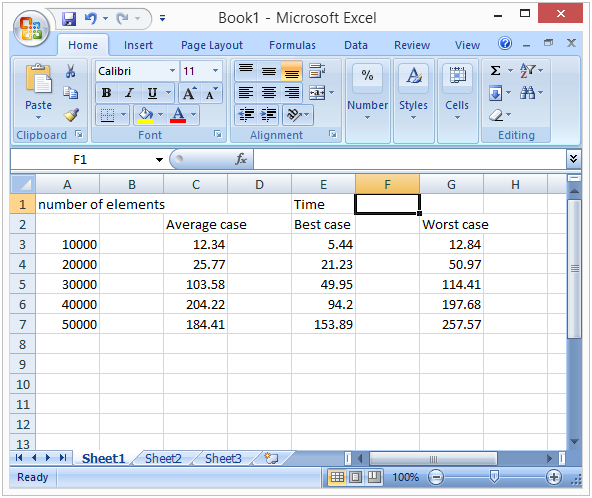
\includegraphics{bubbledata.png}

\hspace{5cm}fig: Table of Time Complexity of Bubble Sort.

\subsection{Time Complexity Graph of BUBBLE-SORT}

The following graph represents time complexity of BUBBLE-SORT.

\vspace{1cm}

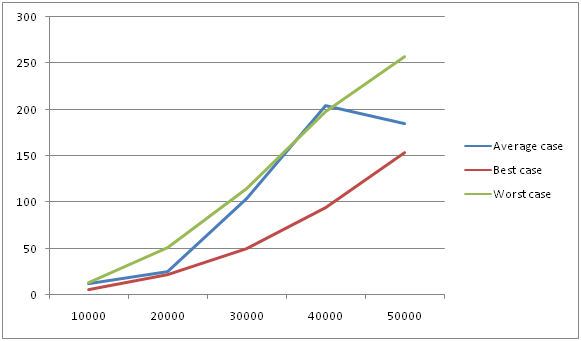
\includegraphics{bubble sort.png}

\hspace{5cm}fig: Time complexity of BUBBLE-SORT.

\section{Quick Sort}

Quick Sort, like Merge Sort, applies the divide and conquer paradigm. Here is the three-step divide and conquer process for sorting a typical subarray $A[p..r]$.

\textbf{Divide:} Partition the array $A[p..r]$ into two (possible empty) subarrays $A[p..q-1]$ and $A[q+1..r]$ such that each element of $A[p..q-1]$ is less than or equal to $A[q]$, which is, in turn, less than or equal to each element of $A[q+1..r]$. Compute the index \textit{q} as part of this partitioning procedure.

\textbf{Conquer:} Sort the two subarrays $A[p..q-1]$ and $A[q+1..r]$ by recursive calls to quick sort.

\textbf{Combine:} Because the subarrays are already sorted, no work is needed to combine them: the entire array $A[p..r]$ is now sorted.

\subsection{Algorithm of Quick Sort}

The following procedure implements quicksort:

\vspace{1cm}

$QUICKSORT(A,p,r)$

1\hspace{0.5cm}$\textbf{if}\hspace{0.2cm}p<r$

2\hspace{1cm}$q=PARTITION(A,p,r)$

3\hspace{1cm}$QUICKSORT(A,p,q-1)$

4\hspace{1cm}$QUICKSORT(A,q+1,r)$

\vspace{0.5cm}

\textbf{Partitioning the array}

\vspace{0.5cm}

The key to the algorithm is the $PARTITIONING$ procedure, which rearranges the subarray $A[p..r]$ in place.

\vspace{0.5cm}

$PARTITION(A,p,r)$

1\hspace{0.5cm}$x=A[r]$

2\hspace{0.5cm}$i=p-1$

3\hspace{0.5cm}\textbf{for} $j=p$  \textbf{to} $r-1$

4\hspace{1cm} \textbf{if} $A[j] \leq x$

5\hspace{1.5cm} $i=i+1$

6\hspace{1.5cm} exchange $A[i]$ with $A[j]$

7\hspace{0.5cm}exchange $A[i+1]$ with $A[r]$

8\hspace{0.5cm}\textbf{return} $i+1$

\subsection{Time Complexity of Quick Sort}

The running time of quick sort is similar at best and average case, but it is larger at worst case.

\vspace{0.5cm}

\textbf{Average case:} The running time is $O(nlgn)$.

\textbf{Best case:} The running time is $O(nlgn)$.

\textbf{Worst case:} The running time is $O(n^2)$.


\vspace{0.5cm}

Here is the Time Complexity Chart of Quick Sort:

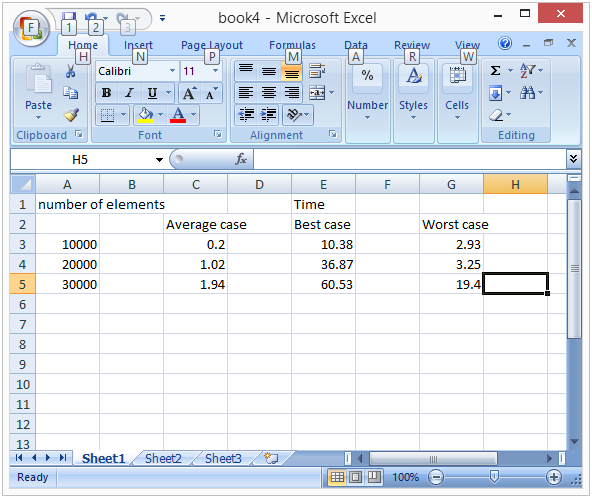
\includegraphics{quickdata.png}

\hspace{5cm}fig: Time Complexity chart of Quick Sort.

\subsection{Time Complexity Graph of Quick Sort}

From chart, we draw a graph that represents the efficiency of Quick Sort algorithm.

\vspace{1cm}

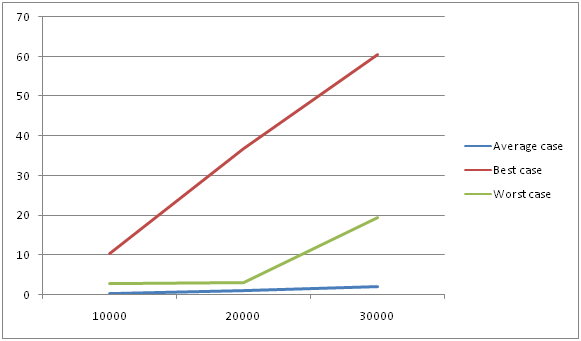
\includegraphics{quicksort.png}

\hspace{5cm}fig: Time Complexity graph of quick sort.

\section{Heap Sort}

Like merge sort, but unlike insertion sort, heapsort's running time is $O(n lgn)$. Like insertion sort, but unlike merge sort, heapsort sorts in place: only a constant number of array elements are stored outside the input array at any time. 

Heapsort also introduces another algorithm design technique: using a data structure, in this case one we call a \textbf{heap}, to manage information. 

\subsection{Algorithm of Heap Sort}


$MAX-HEAPIFY(A,i)$

1\hspace{0.5cm}$l=LEFT(i)$

2\hspace{0.5cm}$r=RIGHT(i)$

3\hspace{0.5cm}\textbf{if} $l \leq A.heap-size$ and $A[l]>A[i]$

4\hspace{1cm}$largest=l$

5\hspace{0.5cm}\textbf{else} $largest=i$

6\hspace{0.5cm}\textbf{if} $r \leq A.heap-size$ and $A[r]>A[largest]$

7\hspace{1cm}$largest=r$

8\hspace{0.5cm}\textbf{if} $largest \neq i$

9\hspace{1cm}exchange $A[i]$ with $A[largest]$

10\hspace{1cm}$MAX-HEAPIFY(A,largest)$

\vspace{1cm}

$BUILD-MAX-HEAP(A)$

1\hspace{0.5cm}\textit{A.heap-size}=\textit{A.length}

2\hspace{0.5cm}\textbf{for} $i=[A.length/2]$ \textbf{downto} 1

3\hspace{1cm}$MAX-HEAPIFY(A,i)$

\vspace{1cm}

$HEAPSORT(A)$

1\hspace{0.5cm}$BUILD-MAX-HEAP(A)$

2\hspace{0.5cm}\textbf{for} $i=A.length$ \textbf{downto} 2

3\hspace{1cm}exchange $A[1]$ with $A[i]$

4\hspace{1cm}\textit{A.heap-size}=\textit{A.heap-size}-1

5\hspace{1cm}$MAX-HEAPIFY(A,1)$

\subsection{Time Complexity of Heap Sort}

The Time complexity of Heap sort is not so complex. The running time of Heao sort is $O(nlgn)$. This is same for the best, average and worst case.

\textbf{Chart for Time Complexity}

Here is the table that contains the data of running time and number of elements.

\vspace{1cm}


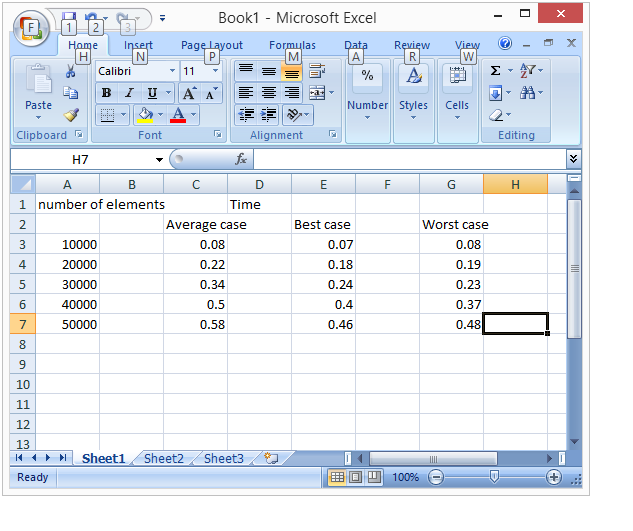
\includegraphics{heapdata.png}

\hspace{5cm}fig: Time Complexity chart.

\subsection{Time Complexity Graph}

Here is the graph that represents the time complexity graph in Heap-Sort.

\vspace{1cm}

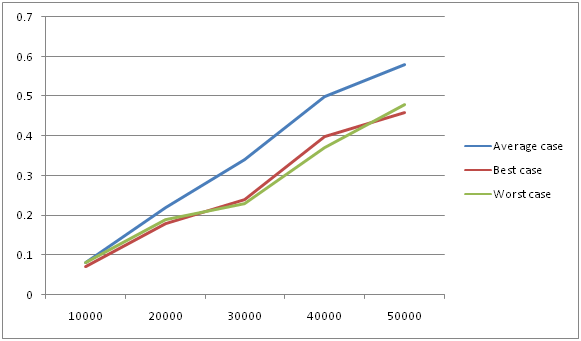
\includegraphics{heapsort.png}

\hspace{5cm}fig: Time Complexity graph of Heap-Sort.










\end{document}